\section{Setting Preferences} \label{sec:preferences}

Use Morpho preferences to select a DataONE
Member Node, customize the look and feel
of the application, and adjust settings that affect logging and
debugging. The advanced tab allows you set a DataONE Coordinating Node 
and import a client certificate for identity providers who do not 
yet support authentication within Morpho. 
Select ``Set preferences...'' under the File menu to open the
Morpho Preferences screen (\autoref{fig:dialog-preferences}).

\begin{figure}
  \centering
    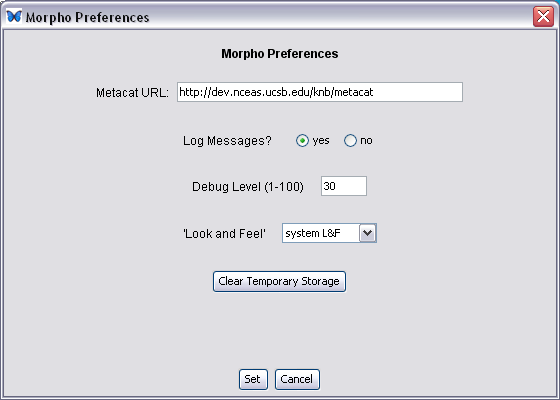
\includegraphics[width=0.7\textwidth]{images/dialog-preferences.png}
  \caption{The Morpho Preferences at the default settings.}
  \label{fig:dialog-preferences}
\end{figure}

\paragraph{Member Node URL} The Member Node URL contains the URL of the specific
DataONE Member Node to which data and metadata will be uploaded. By default, the 
Member Node URL points to the KNB Member Node which accepts user-submitted 
data packages from a wide variety of disciplines. Select a different Member Node 
if your content should primarily be housed on that specific node.
Advanced users can enter a Member Node URL directly if their node is not yet 
registered and available in the list.

\paragraph{Log Messages} The Log Messages preference, when set to ``yes'' (the
default), specifies that error messages be written to a log file. The
log file is called ``stderr.log'' and can be found in the Morpho startup
directory. If you are experiencing problems with the application,
examining the log file (or sending it to Morpho developers to examine)
may provide clues to the cause. Note that the log file is rewritten
every time Morpho starts up. You must rename the file if you want to
save it.

\paragraph{Debug Level (1-100)} The debug level (set to 30 by default)
configures the debugging level used to log. A level of 1 returns only
the most severe errors. A level of 100 returns every possible error.

\paragraph{Look and Feel} Select an option from the drop-down menu.
``system L\&F'' (the default) instructs Morpho to mimic the look of the
current operating system (e.g., Windows, Mac, etc) ``kunststoff'' is a
customized look-and-feel created for Java applications.

\paragraph{Clear Temporary Storage} The ``Clear Temporary Storage''
option empties the Morpho cache, which contains downloaded data sets.
Under most circumstances, you do not need to use this option. However,
if you have downloaded many large data sets and are running low on hard
drive space, you may wish to use this option. Note that when you clear
the cache, Morpho must re-download each data set the next time you
require it.

\begin{figure}
  \centering
    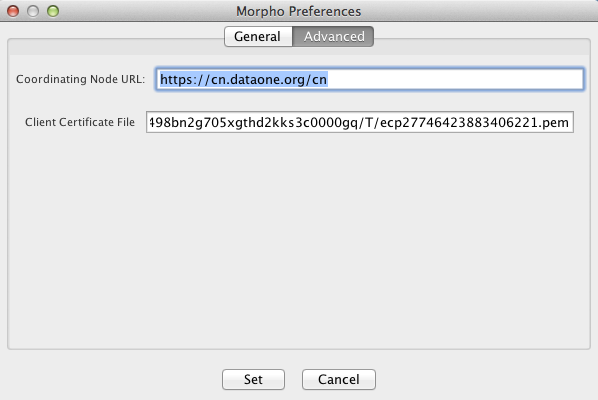
\includegraphics[width=0.7\textwidth]{images/dialog-preferences-advanced.png}
  \caption{Advanced Morpho Preferences}
  \label{fig:dialog-preferences-advanced}
\end{figure}

\paragraph{Coordinating Node URL} The Coordinating Node URL contains the URL 
of the DataONE Coordinating Node that is instrumental in managing data replication, 
user accounts, and other essential DataONE infrastructure requirements.
where data are stored. By default, the Coordinating Node URL points to the
production DataONE environment. Change the default only if you are testing a new feature or 
are an advanced user.

\paragraph{Client Certificate File} If your identity provider is not listed in 
the authentication interface, you can import a client certificate to be used 
for all communication with the Member Node and the Coordinating Node. Typically, users 
will authenticate with their IdP from within Morpho, but not all CILogon identity providers 
support this extended protocol (notably, Google). This value applies only to the profile in 
use when it is set so that multiple profiles can use different client certificates as needed.